\chapter{Consultas en árboles}

\index{consultas en árboles}

En este capítulo veremos técnicas para procesar consultas en
subárboles y caminos de un árbol con raíz. Por ejemplo, tales
consultas pueden ser:
\begin{itemize}
    \item ¿cuál es el $k$-ésimo ancestro de un nodo?
    \item ¿cuál es la suma de valores en el subárbol de un nodo?
    \item ¿cuál es la suma de valores en un camino entre dos nodos?
    \item ¿cuál es el ancestro común más bajo de dos nodos?
\end{itemize}

\section{Encontrar ancestros}

\index{ancestro}

El $k$-ésimo \key{ancestro} de un nodo $x$ en un árbol con raíz es el
nodo que alcanzaremos si nos movemos $k$ niveles hacia arriba desde $x$.
Definamos $\texttt{ancestro}(x,k)$ como el $k$-ésimo ancestro de un nodo
$x$ (o $0$ si tal ancestro no existe). Por ejemplo, en el siguiente árbol,
$\texttt{ancestro}(2,1)=1$ y $\texttt{ancestro}(8,2)=4$.
\begin{center}
    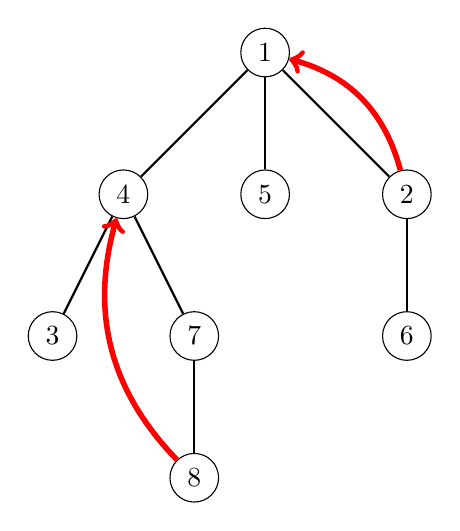
\begin{tikzpicture}[scale=0.9]
        \node[draw, circle] (1) at (0,3) {$1$};
        \node[draw, circle] (2) at (2,1) {$2$};
        \node[draw, circle] (3) at (-2,1) {$4$};
        \node[draw, circle] (4) at (0,1) {$5$};
        \node[draw, circle] (5) at (2,-1) {$6$};
        \node[draw, circle] (6) at (-3,-1) {$3$};
        \node[draw, circle] (7) at (-1,-1) {$7$};
        \node[draw, circle] (8) at (-1,-3) {$8$};
        \path[draw,thick,-] (1) -- (2);
        \path[draw,thick,-] (1) -- (3);
        \path[draw,thick,-] (1) -- (4);
        \path[draw,thick,-] (2) -- (5);
        \path[draw,thick,-] (3) -- (6);
        \path[draw,thick,-] (3) -- (7);
        \path[draw,thick,-] (7) -- (8);

        \path[draw=red,thick,->,line width=2pt] (8) edge [bend left] (3);
        \path[draw=red,thick,->,line width=2pt] (2) edge [bend right] (1);
    \end{tikzpicture}
\end{center}

Una manera fácil de calcular cualquier valor de $\texttt{ancestro}(x,k)$
es realizar una secuencia de $k$ movimientos en el árbol. No obstante,
la complejidad temporal de este método es $O(k)$, que puede ser lento,
porque un árbol de $n$ nodos puede contener una cadena de $n$ nodos
en el peor caso.

Afortunadamente, utilizando una técnica similar a aquella del Capítulo
16.3, cualquier valor de $\texttt{ancestro}(x,k)$ puede ser calculado
eficientemente en $O(\log k)$ luego de un preprocesamiento.
La idea es precalcular todos los valores de $\texttt{ancestro}(x,k)$
donde $k \le n$ sea una potencia de 2. Por ejemplo, los valores para
el árbol de arriba son los siguientes:

\begin{center}
    \begin{tabular}{r|rrrrrrrrr}
        $x$                      & 1 & 2 & 3 & 4 & 5 & 6 & 7 & 8 \\
        \hline
        $\texttt{ancestor}(x,1)$ & 0 & 1 & 4 & 1 & 1 & 2 & 4 & 7 \\
        $\texttt{ancestor}(x,2)$ & 0 & 0 & 1 & 0 & 0 & 1 & 1 & 4 \\
        $\texttt{ancestor}(x,4)$ & 0 & 0 & 0 & 0 & 0 & 0 & 0 & 0 \\
        $\cdots$                                                 \\
    \end{tabular}
\end{center}

El preprocesamiento tarda $O(n \log n)$, porque se calculan $O(\log n)$
valores por cada nodo. Luego de esto, cada valor de
$\texttt{ancestro}(x,k)$ puede calcularse en $O(\log k)$ si
representamos $k$ como una suma donde cada término es una potencia de 2.

\section{Subárboles y caminos}

\index{arreglo de recorrido del árbol}

Un \key{arreglo de recorrido del árbol} contiene los nodos de un
árbol con raíz en el orden en que los visita una búsqueda en
profundidad. Por ejemplo, en el árbol
\begin{center}
    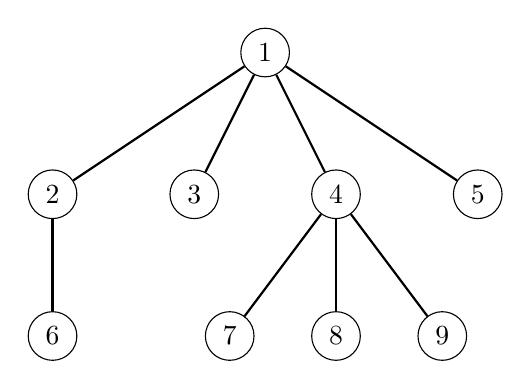
\begin{tikzpicture}[scale=0.9]
        \node[draw, circle] (1) at (0,3) {$1$};
        \node[draw, circle] (2) at (-3,1) {$2$};
        \node[draw, circle] (3) at (-1,1) {$3$};
        \node[draw, circle] (4) at (1,1) {$4$};
        \node[draw, circle] (5) at (3,1) {$5$};
        \node[draw, circle] (6) at (-3,-1) {$6$};
        \node[draw, circle] (7) at (-0.5,-1) {$7$};
        \node[draw, circle] (8) at (1,-1) {$8$};
        \node[draw, circle] (9) at (2.5,-1) {$9$};

        \path[draw,thick,-] (1) -- (2);
        \path[draw,thick,-] (1) -- (3);
        \path[draw,thick,-] (1) -- (4);
        \path[draw,thick,-] (1) -- (5);
        \path[draw,thick,-] (2) -- (6);
        \path[draw,thick,-] (4) -- (7);
        \path[draw,thick,-] (4) -- (8);
        \path[draw,thick,-] (4) -- (9);
    \end{tikzpicture}
\end{center}
una búsqueda en profundidad procede de la siguiente manera:
\begin{center}
    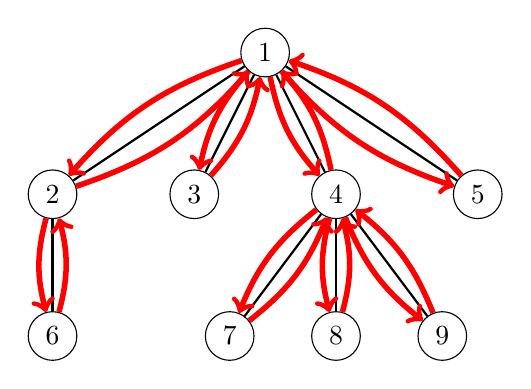
\begin{tikzpicture}[scale=0.9]
        \node[draw, circle] (1) at (0,3) {$1$};
        \node[draw, circle] (2) at (-3,1) {$2$};
        \node[draw, circle] (3) at (-1,1) {$3$};
        \node[draw, circle] (4) at (1,1) {$4$};
        \node[draw, circle] (5) at (3,1) {$5$};
        \node[draw, circle] (6) at (-3,-1) {$6$};
        \node[draw, circle] (7) at (-0.5,-1) {$7$};
        \node[draw, circle] (8) at (1,-1) {$8$};
        \node[draw, circle] (9) at (2.5,-1) {$9$};

        \path[draw,thick,-] (1) -- (2);
        \path[draw,thick,-] (1) -- (3);
        \path[draw,thick,-] (1) -- (4);
        \path[draw,thick,-] (1) -- (5);
        \path[draw,thick,-] (2) -- (6);
        \path[draw,thick,-] (4) -- (7);
        \path[draw,thick,-] (4) -- (8);
        \path[draw,thick,-] (4) -- (9);

        \path[draw=red,thick,->,line width=2pt] (1) edge [bend right=15] (2);
        \path[draw=red,thick,->,line width=2pt] (2) edge [bend right=15] (6);
        \path[draw=red,thick,->,line width=2pt] (6) edge [bend right=15] (2);
        \path[draw=red,thick,->,line width=2pt] (2) edge [bend right=15] (1);
        \path[draw=red,thick,->,line width=2pt] (1) edge [bend right=15] (3);
        \path[draw=red,thick,->,line width=2pt] (3) edge [bend right=15] (1);
        \path[draw=red,thick,->,line width=2pt] (1) edge [bend right=15] (4);
        \path[draw=red,thick,->,line width=2pt] (4) edge [bend right=15] (7);
        \path[draw=red,thick,->,line width=2pt] (7) edge [bend right=15] (4);
        \path[draw=red,thick,->,line width=2pt] (4) edge [bend right=15] (8);
        \path[draw=red,thick,->,line width=2pt] (8) edge [bend right=15] (4);
        \path[draw=red,thick,->,line width=2pt] (4) edge [bend right=15] (9);
        \path[draw=red,thick,->,line width=2pt] (9) edge [bend right=15] (4);
        \path[draw=red,thick,->,line width=2pt] (4) edge [bend right=15] (1);
        \path[draw=red,thick,->,line width=2pt] (1) edge [bend right=15] (5);
        \path[draw=red,thick,->,line width=2pt] (5) edge [bend right=15] (1);

    \end{tikzpicture}
\end{center}
Por ende, el arreglo de recorrido del árbol es el siguiente:
\begin{center}
    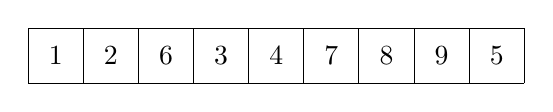
\begin{tikzpicture}[scale=0.7]
        \draw (0,0) grid (9,1);

        \node at (0.5,0.5) {$1$};
        \node at (1.5,0.5) {$2$};
        \node at (2.5,0.5) {$6$};
        \node at (3.5,0.5) {$3$};
        \node at (4.5,0.5) {$4$};
        \node at (5.5,0.5) {$7$};
        \node at (6.5,0.5) {$8$};
        \node at (7.5,0.5) {$9$};
        \node at (8.5,0.5) {$5$};
        %
        % \footnotesize
        % \node at (0.5,1.4) {$1$};
        % \node at (1.5,1.4) {$2$};
        % \node at (2.5,1.4) {$3$};
        % \node at (3.5,1.4) {$4$};
        % \node at (4.5,1.4) {$5$};
        % \node at (5.5,1.4) {$6$};
        % \node at (6.5,1.4) {$7$};
        % \node at (7.5,1.4) {$8$};
        % \node at (8.5,1.4) {$9$};
    \end{tikzpicture}
\end{center}

\subsubsection{Consultas en subárboles}

Cada subárbol de un árbol corresponde a un subarreglo del arreglo
de recorrido del árbol tal que el primer elemento del subarreglo
sea el nodo raíz. Por ejemplo, el siguiente subarreglo contiene
los nodos del subárbol del nodo $4$:
\begin{center}
    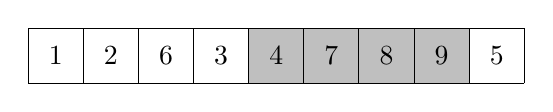
\begin{tikzpicture}[scale=0.7]
        \fill[color=lightgray] (4,0) rectangle (8,1);
        \draw (0,0) grid (9,1);

        \node at (0.5,0.5) {$1$};
        \node at (1.5,0.5) {$2$};
        \node at (2.5,0.5) {$6$};
        \node at (3.5,0.5) {$3$};
        \node at (4.5,0.5) {$4$};
        \node at (5.5,0.5) {$7$};
        \node at (6.5,0.5) {$8$};
        \node at (7.5,0.5) {$9$};
        \node at (8.5,0.5) {$5$};
        %
        % \footnotesize
        % \node at (0.5,1.4) {$1$};
        % \node at (1.5,1.4) {$2$};
        % \node at (2.5,1.4) {$3$};
        % \node at (3.5,1.4) {$4$};
        % \node at (4.5,1.4) {$5$};
        % \node at (5.5,1.4) {$6$};
        % \node at (6.5,1.4) {$7$};
        % \node at (7.5,1.4) {$8$};
        % \node at (8.5,1.4) {$9$};
    \end{tikzpicture}
\end{center}

Utilizando este hecho, podemos eficientemente procesar consultas
relacionadas a los subárboles de un árbol. Por ejemplo, considera
un problema donde cada nodo es asignado un valor, y nuestra tarea
es llevar a cabo estas consultas:
\begin{itemize}
    \item actualizar el valor de un nodo
    \item calcular la suma de valores en el subárbol de un nodo
\end{itemize}

Considera el siguiente árbol donde los números azules son los valores
de los nodos. Por ejemplo, la suma del subárbol del nodo $4$ es
$3+4+3+1=11$.

\begin{center}
    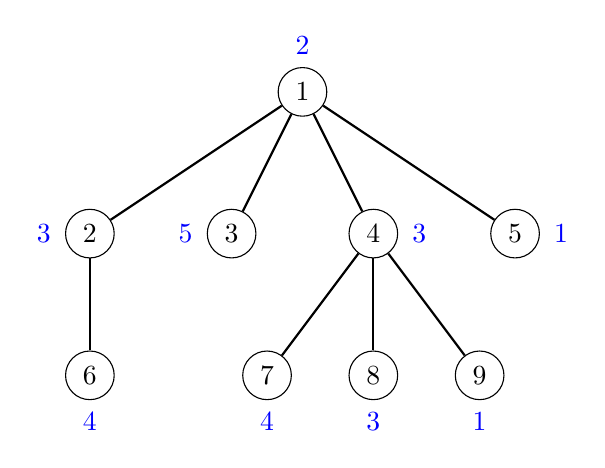
\begin{tikzpicture}[scale=0.9]
        \node[draw, circle] (1) at (0,3) {$1$};
        \node[draw, circle] (2) at (-3,1) {$2$};
        \node[draw, circle] (3) at (-1,1) {$3$};
        \node[draw, circle] (4) at (1,1) {$4$};
        \node[draw, circle] (5) at (3,1) {$5$};
        \node[draw, circle] (6) at (-3,-1) {$6$};
        \node[draw, circle] (7) at (-0.5,-1) {$7$};
        \node[draw, circle] (8) at (1,-1) {$8$};
        \node[draw, circle] (9) at (2.5,-1) {$9$};

        \path[draw,thick,-] (1) -- (2);
        \path[draw,thick,-] (1) -- (3);
        \path[draw,thick,-] (1) -- (4);
        \path[draw,thick,-] (1) -- (5);
        \path[draw,thick,-] (2) -- (6);
        \path[draw,thick,-] (4) -- (7);
        \path[draw,thick,-] (4) -- (8);
        \path[draw,thick,-] (4) -- (9);

        \node[color=blue] at (0,3+0.65) {2};
        \node[color=blue] at (-3-0.65,1) {3};
        \node[color=blue] at (-1-0.65,1) {5};
        \node[color=blue] at (1+0.65,1) {3};
        \node[color=blue] at (3+0.65,1) {1};
        \node[color=blue] at (-3,-1-0.65) {4};
        \node[color=blue] at (-0.5,-1-0.65) {4};
        \node[color=blue] at (1,-1-0.65) {3};
        \node[color=blue] at (2.5,-1-0.65) {1};
    \end{tikzpicture}
\end{center}

La idea es construir un arreglo de recorrido de árbol que contenga
tres valores por cada nodo: su identificador, el tamaño de su subárbol,
y el valor del nodo. Por ejemplo, el arreglo para el árbol anterior
es el siguiente:

\begin{center}
    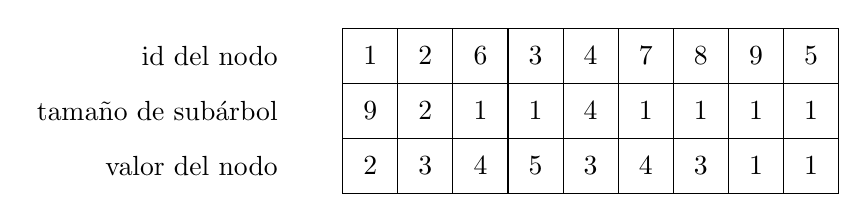
\begin{tikzpicture}[scale=0.7]
        \draw (0,1) grid (9,-2);

        \node[left] at (-1,0.5) {id del nodo};
        \node[left] at (-1,-0.5) {tamaño de subárbol};
        \node[left] at (-1,-1.5) {valor del nodo};

        \node at (0.5,0.5) {$1$};
        \node at (1.5,0.5) {$2$};
        \node at (2.5,0.5) {$6$};
        \node at (3.5,0.5) {$3$};
        \node at (4.5,0.5) {$4$};
        \node at (5.5,0.5) {$7$};
        \node at (6.5,0.5) {$8$};
        \node at (7.5,0.5) {$9$};
        \node at (8.5,0.5) {$5$};

        \node at (0.5,-0.5) {$9$};
        \node at (1.5,-0.5) {$2$};
        \node at (2.5,-0.5) {$1$};
        \node at (3.5,-0.5) {$1$};
        \node at (4.5,-0.5) {$4$};
        \node at (5.5,-0.5) {$1$};
        \node at (6.5,-0.5) {$1$};
        \node at (7.5,-0.5) {$1$};
        \node at (8.5,-0.5) {$1$};

        \node at (0.5,-1.5) {$2$};
        \node at (1.5,-1.5) {$3$};
        \node at (2.5,-1.5) {$4$};
        \node at (3.5,-1.5) {$5$};
        \node at (4.5,-1.5) {$3$};
        \node at (5.5,-1.5) {$4$};
        \node at (6.5,-1.5) {$3$};
        \node at (7.5,-1.5) {$1$};
        \node at (8.5,-1.5) {$1$};
        %
        % \footnotesize
        % \node at (0.5,1.4) {$1$};
        % \node at (1.5,1.4) {$2$};
        % \node at (2.5,1.4) {$3$};
        % \node at (3.5,1.4) {$4$};
        % \node at (4.5,1.4) {$5$};
        % \node at (5.5,1.4) {$6$};
        % \node at (6.5,1.4) {$7$};
        % \node at (7.5,1.4) {$8$};
        % \node at (8.5,1.4) {$9$};
    \end{tikzpicture}
\end{center}

Utilizando este arreglo, podemos calcular la suma de valores en
cualquier subárbol si primero encontramos el tamaño del subárbol
y luego los valores de los nodos correspondientes. Por ejemplo,
los valores en el subárbol del nodo $4$ pueden encontrarse así:

\begin{center}
    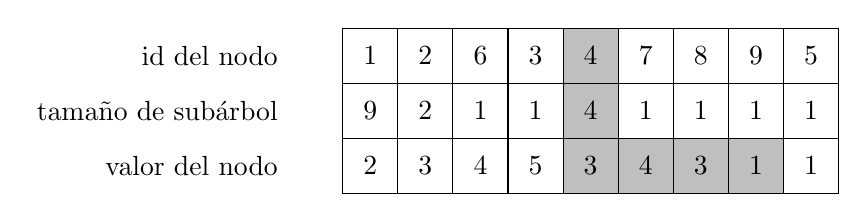
\begin{tikzpicture}[scale=0.7]
        \fill[color=lightgray] (4,1) rectangle (5,0);
        \fill[color=lightgray] (4,0) rectangle (5,-1);
        \fill[color=lightgray] (4,-1) rectangle (8,-2);
        \draw (0,1) grid (9,-2);

        \node[left] at (-1,0.5) {id del nodo};
        \node[left] at (-1,-0.5) {tamaño de subárbol};
        \node[left] at (-1,-1.5) {valor del nodo};

        \node at (0.5,0.5) {$1$};
        \node at (1.5,0.5) {$2$};
        \node at (2.5,0.5) {$6$};
        \node at (3.5,0.5) {$3$};
        \node at (4.5,0.5) {$4$};
        \node at (5.5,0.5) {$7$};
        \node at (6.5,0.5) {$8$};
        \node at (7.5,0.5) {$9$};
        \node at (8.5,0.5) {$5$};

        \node at (0.5,-0.5) {$9$};
        \node at (1.5,-0.5) {$2$};
        \node at (2.5,-0.5) {$1$};
        \node at (3.5,-0.5) {$1$};
        \node at (4.5,-0.5) {$4$};
        \node at (5.5,-0.5) {$1$};
        \node at (6.5,-0.5) {$1$};
        \node at (7.5,-0.5) {$1$};
        \node at (8.5,-0.5) {$1$};

        \node at (0.5,-1.5) {$2$};
        \node at (1.5,-1.5) {$3$};
        \node at (2.5,-1.5) {$4$};
        \node at (3.5,-1.5) {$5$};
        \node at (4.5,-1.5) {$3$};
        \node at (5.5,-1.5) {$4$};
        \node at (6.5,-1.5) {$3$};
        \node at (7.5,-1.5) {$1$};
        \node at (8.5,-1.5) {$1$};
        %
        % \footnotesize
        % \node at (0.5,1.4) {$1$};
        % \node at (1.5,1.4) {$2$};
        % \node at (2.5,1.4) {$3$};
        % \node at (3.5,1.4) {$4$};
        % \node at (4.5,1.4) {$5$};
        % \node at (5.5,1.4) {$6$};
        % \node at (6.5,1.4) {$7$};
        % \node at (7.5,1.4) {$8$};
        % \node at (8.5,1.4) {$9$};
    \end{tikzpicture}
\end{center}

Para realizar las consultas eficientemente, es suficiente almacenar
los valores de los nodos en un árbol binario indexado o de segmentos.
Luego de esto, podemos actualizar un valor y calcular la suma de valores
en $O(\log n)$.

\subsubsection{Consultas en caminos}

Utilizando un arreglo de recorrido del árbol, también podemos
calcular sumas de valores eficientemente en caminos desde el nodo raíz
a cualquier nodo del árbol. Considera un problema donde nuestra tarea
es soportar las siguientes consultas:
\begin{itemize}
    \item modificar el valor de un nodo
    \item calcular la suma de valores en un camino de la raíz a un nodo
\end{itemize}

Por ejemplo, en el siguiente árbol, la suma de valores de la raíz al
nodo 7 es $4+5+5=14$:

\begin{center}
    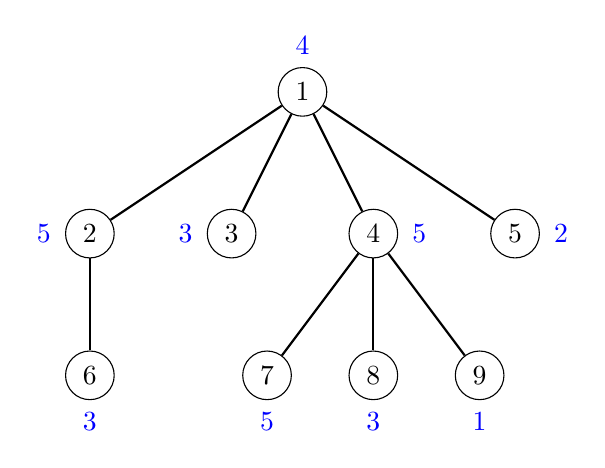
\begin{tikzpicture}[scale=0.9]
        \node[draw, circle] (1) at (0,3) {$1$};
        \node[draw, circle] (2) at (-3,1) {$2$};
        \node[draw, circle] (3) at (-1,1) {$3$};
        \node[draw, circle] (4) at (1,1) {$4$};
        \node[draw, circle] (5) at (3,1) {$5$};
        \node[draw, circle] (6) at (-3,-1) {$6$};
        \node[draw, circle] (7) at (-0.5,-1) {$7$};
        \node[draw, circle] (8) at (1,-1) {$8$};
        \node[draw, circle] (9) at (2.5,-1) {$9$};

        \path[draw,thick,-] (1) -- (2);
        \path[draw,thick,-] (1) -- (3);
        \path[draw,thick,-] (1) -- (4);
        \path[draw,thick,-] (1) -- (5);
        \path[draw,thick,-] (2) -- (6);
        \path[draw,thick,-] (4) -- (7);
        \path[draw,thick,-] (4) -- (8);
        \path[draw,thick,-] (4) -- (9);

        \node[color=blue] at (0,3+0.65) {4};
        \node[color=blue] at (-3-0.65,1) {5};
        \node[color=blue] at (-1-0.65,1) {3};
        \node[color=blue] at (1+0.65,1) {5};
        \node[color=blue] at (3+0.65,1) {2};
        \node[color=blue] at (-3,-1-0.65) {3};
        \node[color=blue] at (-0.5,-1-0.65) {5};
        \node[color=blue] at (1,-1-0.65) {3};
        \node[color=blue] at (2.5,-1-0.65) {1};
    \end{tikzpicture}
\end{center}

Podemos resolver este problema como anteriormente, pero ahora cada valor
en la última fila del arreglo es la suma de valores de un camino desde
la raíz al nodo. Por ejemplo, el siguiente arreglo corresponde al
árbol de arriba:
\begin{center}
    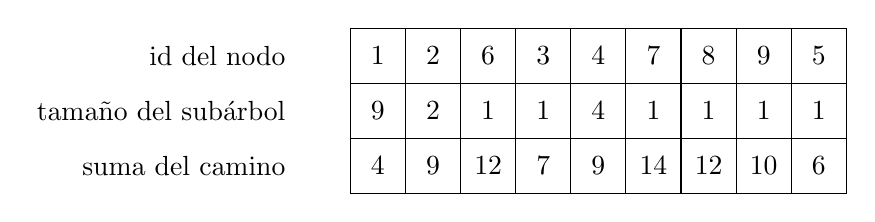
\begin{tikzpicture}[scale=0.7]
        \draw (0,1) grid (9,-2);

        \node[left] at (-1,0.5) {id del nodo};
        \node[left] at (-1,-0.5) {tamaño del subárbol};
        \node[left] at (-1,-1.5) {suma del camino};

        \node at (0.5,0.5) {$1$};
        \node at (1.5,0.5) {$2$};
        \node at (2.5,0.5) {$6$};
        \node at (3.5,0.5) {$3$};
        \node at (4.5,0.5) {$4$};
        \node at (5.5,0.5) {$7$};
        \node at (6.5,0.5) {$8$};
        \node at (7.5,0.5) {$9$};
        \node at (8.5,0.5) {$5$};

        \node at (0.5,-0.5) {$9$};
        \node at (1.5,-0.5) {$2$};
        \node at (2.5,-0.5) {$1$};
        \node at (3.5,-0.5) {$1$};
        \node at (4.5,-0.5) {$4$};
        \node at (5.5,-0.5) {$1$};
        \node at (6.5,-0.5) {$1$};
        \node at (7.5,-0.5) {$1$};
        \node at (8.5,-0.5) {$1$};

        \node at (0.5,-1.5) {$4$};
        \node at (1.5,-1.5) {$9$};
        \node at (2.5,-1.5) {$12$};
        \node at (3.5,-1.5) {$7$};
        \node at (4.5,-1.5) {$9$};
        \node at (5.5,-1.5) {$14$};
        \node at (6.5,-1.5) {$12$};
        \node at (7.5,-1.5) {$10$};
        \node at (8.5,-1.5) {$6$};
    \end{tikzpicture}
\end{center}

Cuando el valor de un nodo se aumenta por $x$, la suma de todos los
nodos en su subárbol aumenta por $x$. Por ejemplo, si el valor de nodo 4
aumenta por 1, el arreglo cambia de la siguiente manera:

\begin{center}
    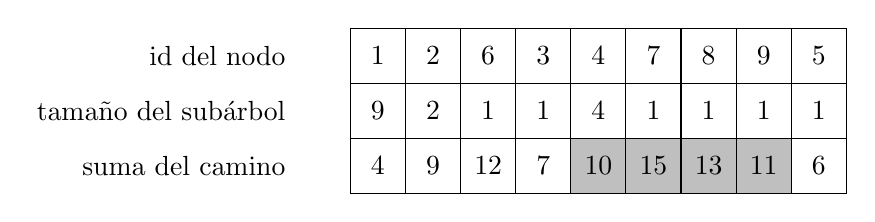
\begin{tikzpicture}[scale=0.7]
        \fill[color=lightgray] (4,-1) rectangle (8,-2);
        \draw (0,1) grid (9,-2);

        \node[left] at (-1,0.5) {id del nodo};
        \node[left] at (-1,-0.5) {tamaño del subárbol};
        \node[left] at (-1,-1.5) {suma del camino};

        \node at (0.5,0.5) {$1$};
        \node at (1.5,0.5) {$2$};
        \node at (2.5,0.5) {$6$};
        \node at (3.5,0.5) {$3$};
        \node at (4.5,0.5) {$4$};
        \node at (5.5,0.5) {$7$};
        \node at (6.5,0.5) {$8$};
        \node at (7.5,0.5) {$9$};
        \node at (8.5,0.5) {$5$};

        \node at (0.5,-0.5) {$9$};
        \node at (1.5,-0.5) {$2$};
        \node at (2.5,-0.5) {$1$};
        \node at (3.5,-0.5) {$1$};
        \node at (4.5,-0.5) {$4$};
        \node at (5.5,-0.5) {$1$};
        \node at (6.5,-0.5) {$1$};
        \node at (7.5,-0.5) {$1$};
        \node at (8.5,-0.5) {$1$};

        \node at (0.5,-1.5) {$4$};
        \node at (1.5,-1.5) {$9$};
        \node at (2.5,-1.5) {$12$};
        \node at (3.5,-1.5) {$7$};
        \node at (4.5,-1.5) {$10$};
        \node at (5.5,-1.5) {$15$};
        \node at (6.5,-1.5) {$13$};
        \node at (7.5,-1.5) {$11$};
        \node at (8.5,-1.5) {$6$};
    \end{tikzpicture}
\end{center}

Por ende, para soportar las dos operaciones, deberíamos ser capaces
de aumentar todos los valores de un rango y acceder a un valor. Esto
puede hacerse en $O(\log n)$ utilizando un árbol binario indexado o
un árbol de segmentos (ver Capítulo 9.4).

\section{Ancestro común más bajo}

\index{ancestro común más bajo}

El \key{ancestro común más bajo} de dos nodos de un árbol con raíz
es el nodo más bajo cuyo subárbol contenga ambos nodos. Un problema
típico es eficientemente procesar consultas que piden encontrar el
ancestro común más bajo de dos nodos.

Por ejemplo, en el siguiente árbol, el ancestro común más bajo de
los nodos 5 y 8 es el nodo 2:
\begin{center}
    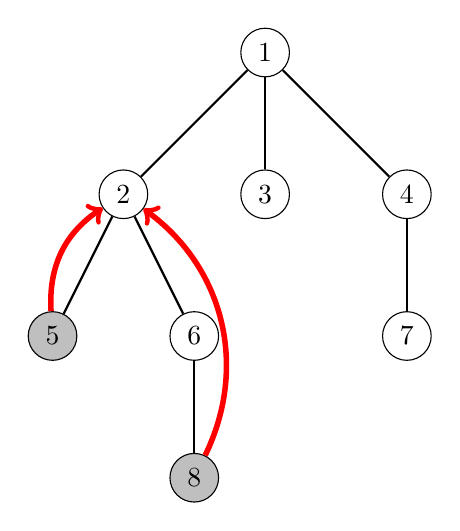
\begin{tikzpicture}[scale=0.9]
        \node[draw, circle] (1) at (0,3) {$1$};
        \node[draw, circle] (2) at (2,1) {$4$};
        \node[draw, circle] (3) at (-2,1) {$2$};
        \node[draw, circle] (4) at (0,1) {$3$};
        \node[draw, circle] (5) at (2,-1) {$7$};
        \node[draw, circle, fill=lightgray] (6) at (-3,-1) {$5$};
        \node[draw, circle] (7) at (-1,-1) {$6$};
        \node[draw, circle, fill=lightgray] (8) at (-1,-3) {$8$};
        \path[draw,thick,-] (1) -- (2);
        \path[draw,thick,-] (1) -- (3);
        \path[draw,thick,-] (1) -- (4);
        \path[draw,thick,-] (2) -- (5);
        \path[draw,thick,-] (3) -- (6);
        \path[draw,thick,-] (3) -- (7);
        \path[draw,thick,-] (7) -- (8);

        \path[draw=red,thick,->,line width=2pt] (6) edge [bend left] (3);
        \path[draw=red,thick,->,line width=2pt] (8) edge [bend right=40] (3);
    \end{tikzpicture}
\end{center}

Ahora veremos dos técnicas eficientes para encontrar el ancestro
común más bajo de dos nodos.

\subsubsection{Método 1}

Una manera de resolver el problema es usando el hecho de que podemos
eficientemente encontrar el $k$-ésimo ancestro de cualquier nodo en el
árbol. Con esto, podemos dividir el problema del ancestro común más
bajo en dos partes.

Utilizamos dos punteros que inicialmente apuntan a los dos nodos cuyo
ancestro común más bajo queremos encontrar. Primero, movemos alguno de
los dos punteros hacia arriba tal que los dos punteros queden en el
mismo nivel.

En la situación de ejemplo, movemos el segundo puntero un nivel hacia
arriba tal que apunte al nodo 6, que se encuentra en el mismo nivel
que el nodo 5:

\begin{center}
    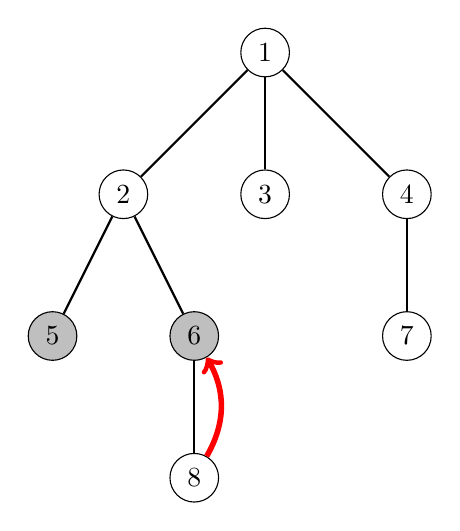
\begin{tikzpicture}[scale=0.9]
        \node[draw, circle] (1) at (0,3) {$1$};
        \node[draw, circle] (2) at (2,1) {$4$};
        \node[draw, circle] (3) at (-2,1) {$2$};
        \node[draw, circle] (4) at (0,1) {$3$};
        \node[draw, circle] (5) at (2,-1) {$7$};
        \node[draw, circle,fill=lightgray] (6) at (-3,-1) {$5$};
        \node[draw, circle,fill=lightgray] (7) at (-1,-1) {$6$};
        \node[draw, circle] (8) at (-1,-3) {$8$};
        \path[draw,thick,-] (1) -- (2);
        \path[draw,thick,-] (1) -- (3);
        \path[draw,thick,-] (1) -- (4);
        \path[draw,thick,-] (2) -- (5);
        \path[draw,thick,-] (3) -- (6);
        \path[draw,thick,-] (3) -- (7);
        \path[draw,thick,-] (7) -- (8);

        \path[draw=red,thick,->,line width=2pt] (8) edge [bend right] (7);
    \end{tikzpicture}
\end{center}

Luego de esto, determinamos el mínimo número de pasos necesarios
para mover los dos punteros hacia arriba tal que apunten
al mismo nodo. El nodo al que apunten los dos punteros luego de esto
es el ancestro común más bajo.

En la situación de ejemplo, es suficiente mover los dos punteros un
paso hacia arriba, hasta el nodo 2, que resulta ser el ancestro común
más bajo:

\begin{center}
    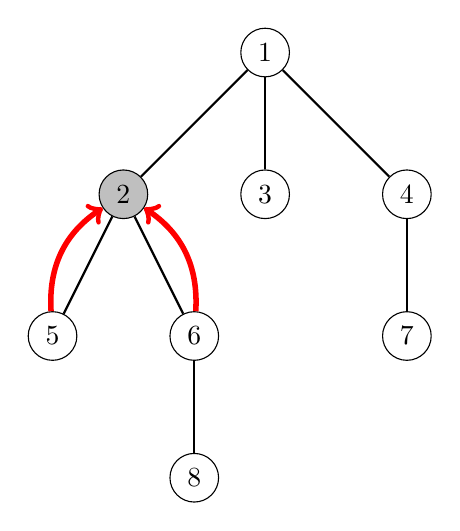
\begin{tikzpicture}[scale=0.9]
        \node[draw, circle] (1) at (0,3) {$1$};
        \node[draw, circle] (2) at (2,1) {$4$};
        \node[draw, circle,fill=lightgray] (3) at (-2,1) {$2$};
        \node[draw, circle] (4) at (0,1) {$3$};
        \node[draw, circle] (5) at (2,-1) {$7$};
        \node[draw, circle] (6) at (-3,-1) {$5$};
        \node[draw, circle] (7) at (-1,-1) {$6$};
        \node[draw, circle] (8) at (-1,-3) {$8$};
        \path[draw,thick,-] (1) -- (2);
        \path[draw,thick,-] (1) -- (3);
        \path[draw,thick,-] (1) -- (4);
        \path[draw,thick,-] (2) -- (5);
        \path[draw,thick,-] (3) -- (6);
        \path[draw,thick,-] (3) -- (7);
        \path[draw,thick,-] (7) -- (8);

        \path[draw=red,thick,->,line width=2pt] (6) edge [bend left] (3);
        \path[draw=red,thick,->,line width=2pt] (7) edge [bend right] (3);
    \end{tikzpicture}
\end{center}

Debido a que las dos fases del algoritmo pueden realizarse en
$O(\log n)$ utilizando información precomputada, podemos encontrar
el ancestro común más bajo de cualquier par de nodos en $O(\log n)$.

\subsubsection{Método 2}

\index{técnica del camino euleriano}

Otra forma de resolver este problema se basa en un arreglo de
recorrido.\footnote{Este algoritmo fue presentado en
    \cite{ben00}. Esta técnica es conocida como la \key{técnica del
        camino euleriano} (o ETT, por \textit{Euler tour technique}).
    \cite{tar84}} Nuevamente, la idea es recorrer los nodos
utilizando una búsqueda en profundidad:

\begin{center}
    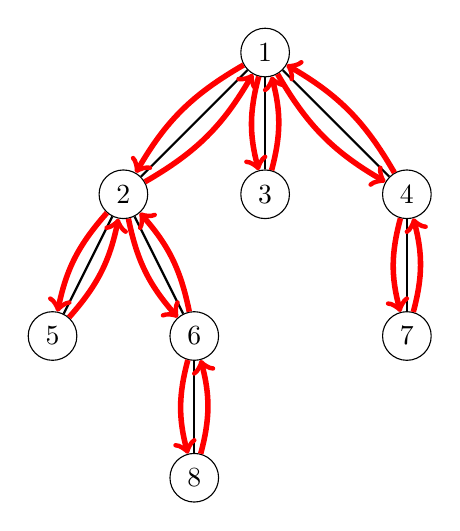
\begin{tikzpicture}[scale=0.9]
        \node[draw, circle] (1) at (0,3) {$1$};
        \node[draw, circle] (2) at (2,1) {$4$};
        \node[draw, circle] (3) at (-2,1) {$2$};
        \node[draw, circle] (4) at (0,1) {$3$};
        \node[draw, circle] (5) at (2,-1) {$7$};
        \node[draw, circle] (6) at (-3,-1) {$5$};
        \node[draw, circle] (7) at (-1,-1) {$6$};
        \node[draw, circle] (8) at (-1,-3) {$8$};
        \path[draw,thick,-] (1) -- (2);
        \path[draw,thick,-] (1) -- (3);
        \path[draw,thick,-] (1) -- (4);
        \path[draw,thick,-] (2) -- (5);
        \path[draw,thick,-] (3) -- (6);
        \path[draw,thick,-] (3) -- (7);
        \path[draw,thick,-] (7) -- (8);

        \path[draw=red,thick,->,line width=2pt] (1) edge [bend right=15] (3);
        \path[draw=red,thick,->,line width=2pt] (3) edge [bend right=15] (6);
        \path[draw=red,thick,->,line width=2pt] (6) edge [bend right=15] (3);
        \path[draw=red,thick,->,line width=2pt] (3) edge [bend right=15] (7);
        \path[draw=red,thick,->,line width=2pt] (7) edge [bend right=15] (8);
        \path[draw=red,thick,->,line width=2pt] (8) edge [bend right=15] (7);
        \path[draw=red,thick,->,line width=2pt] (7) edge [bend right=15] (3);
        \path[draw=red,thick,->,line width=2pt] (3) edge [bend right=15] (1);
        \path[draw=red,thick,->,line width=2pt] (1) edge [bend right=15] (4);
        \path[draw=red,thick,->,line width=2pt] (4) edge [bend right=15] (1);
        \path[draw=red,thick,->,line width=2pt] (1) edge [bend right=15] (2);
        \path[draw=red,thick,->,line width=2pt] (2) edge [bend right=15] (5);
        \path[draw=red,thick,->,line width=2pt] (5) edge [bend right=15] (2);
        \path[draw=red,thick,->,line width=2pt] (2) edge [bend right=15] (1);
    \end{tikzpicture}
\end{center}

No obstante, usamos un arreglo de recorrido de árbol distinto:
añadimos cada nodo al arreglo \emph{siempre} que la búsqueda en
profundidad pase por el nodo, y no solo en la primera visita.
Por lo tanto, un nodo con $k$ hijos aparece $k+1$ veces en el arreglo
y hay un total de $2n-1$ nodos en el arreglo.

Almacenamos dos valores en el arreglo: el identificador del nodo
y la profundidad del nodo en el árbol. El siguiente arreglo
corresponde al árbol de arriba:

\begin{center}
    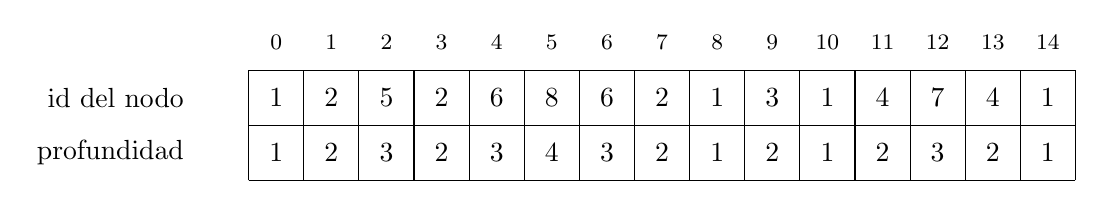
\begin{tikzpicture}[scale=0.7]

        \node[left] at (-1,1.5) {id del nodo};
        \node[left] at (-1,0.5) {profundidad};

        \draw (0,1) grid (15,2);
        \node at (0.5,1.5) {$1$};
        \node at (1.5,1.5) {$2$};
        \node at (2.5,1.5) {$5$};
        \node at (3.5,1.5) {$2$};
        \node at (4.5,1.5) {$6$};
        \node at (5.5,1.5) {$8$};
        \node at (6.5,1.5) {$6$};
        \node at (7.5,1.5) {$2$};
        \node at (8.5,1.5) {$1$};
        \node at (9.5,1.5) {$3$};
        \node at (10.5,1.5) {$1$};
        \node at (11.5,1.5) {$4$};
        \node at (12.5,1.5) {$7$};
        \node at (13.5,1.5) {$4$};
        \node at (14.5,1.5) {$1$};

        \draw (0,0) grid (15,1);
        \node at (0.5,0.5) {$1$};
        \node at (1.5,0.5) {$2$};
        \node at (2.5,0.5) {$3$};
        \node at (3.5,0.5) {$2$};
        \node at (4.5,0.5) {$3$};
        \node at (5.5,0.5) {$4$};
        \node at (6.5,0.5) {$3$};
        \node at (7.5,0.5) {$2$};
        \node at (8.5,0.5) {$1$};
        \node at (9.5,0.5) {$2$};
        \node at (10.5,0.5) {$1$};
        \node at (11.5,0.5) {$2$};
        \node at (12.5,0.5) {$3$};
        \node at (13.5,0.5) {$2$};
        \node at (14.5,0.5) {$1$};

        \footnotesize
        \node at (0.5,2.5) {$0$};
        \node at (1.5,2.5) {$1$};
        \node at (2.5,2.5) {$2$};
        \node at (3.5,2.5) {$3$};
        \node at (4.5,2.5) {$4$};
        \node at (5.5,2.5) {$5$};
        \node at (6.5,2.5) {$6$};
        \node at (7.5,2.5) {$7$};
        \node at (8.5,2.5) {$8$};
        \node at (9.5,2.5) {$9$};
        \node at (10.5,2.5) {$10$};
        \node at (11.5,2.5) {$11$};
        \node at (12.5,2.5) {$12$};
        \node at (13.5,2.5) {$13$};
        \node at (14.5,2.5) {$14$};
    \end{tikzpicture}
\end{center}

Ahora podemos encontrar el ancestro común más bajo de los nodos $a$
y $b$ encontrando el nodo de \emph{mínima profundidad} entre los
nodos $a$ y $b$ en el arreglo. Por ejemplo, el ancestro común más
bajo de los nodos $5$ y $8$ puede encontrarse así:

\begin{center}
    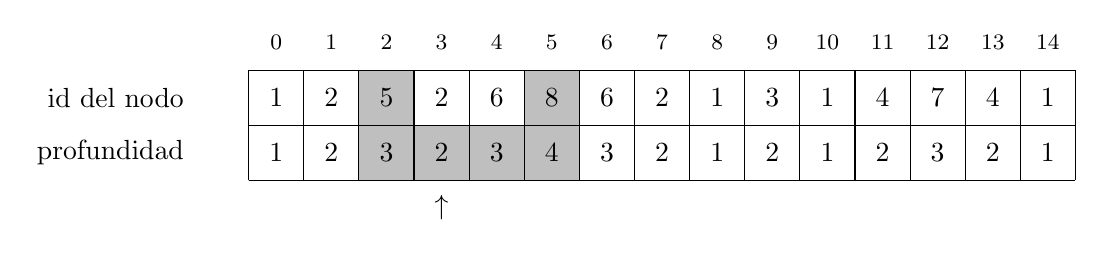
\begin{tikzpicture}[scale=0.7]

        \node[left] at (-1,1.5) {id del nodo};
        \node[left] at (-1,0.5) {profundidad};

        \fill[color=lightgray] (2,1) rectangle (3,2);
        \fill[color=lightgray] (5,1) rectangle (6,2);
        \fill[color=lightgray] (2,0) rectangle (6,1);

        \node at (3.5,-0.5) {$\uparrow$};

        \draw (0,1) grid (15,2);
        \node at (0.5,1.5) {$1$};
        \node at (1.5,1.5) {$2$};
        \node at (2.5,1.5) {$5$};
        \node at (3.5,1.5) {$2$};
        \node at (4.5,1.5) {$6$};
        \node at (5.5,1.5) {$8$};
        \node at (6.5,1.5) {$6$};
        \node at (7.5,1.5) {$2$};
        \node at (8.5,1.5) {$1$};
        \node at (9.5,1.5) {$3$};
        \node at (10.5,1.5) {$1$};
        \node at (11.5,1.5) {$4$};
        \node at (12.5,1.5) {$7$};
        \node at (13.5,1.5) {$4$};
        \node at (14.5,1.5) {$1$};


        \draw (0,0) grid (15,1);
        \node at (0.5,0.5) {$1$};
        \node at (1.5,0.5) {$2$};
        \node at (2.5,0.5) {$3$};
        \node at (3.5,0.5) {$2$};
        \node at (4.5,0.5) {$3$};
        \node at (5.5,0.5) {$4$};
        \node at (6.5,0.5) {$3$};
        \node at (7.5,0.5) {$2$};
        \node at (8.5,0.5) {$1$};
        \node at (9.5,0.5) {$2$};
        \node at (10.5,0.5) {$1$};
        \node at (11.5,0.5) {$2$};
        \node at (12.5,0.5) {$3$};
        \node at (13.5,0.5) {$2$};
        \node at (14.5,0.5) {$1$};

        \footnotesize
        \node at (0.5,2.5) {$0$};
        \node at (1.5,2.5) {$1$};
        \node at (2.5,2.5) {$2$};
        \node at (3.5,2.5) {$3$};
        \node at (4.5,2.5) {$4$};
        \node at (5.5,2.5) {$5$};
        \node at (6.5,2.5) {$6$};
        \node at (7.5,2.5) {$7$};
        \node at (8.5,2.5) {$8$};
        \node at (9.5,2.5) {$9$};
        \node at (10.5,2.5) {$10$};
        \node at (11.5,2.5) {$11$};
        \node at (12.5,2.5) {$12$};
        \node at (13.5,2.5) {$13$};
        \node at (14.5,2.5) {$14$};
    \end{tikzpicture}
\end{center}

El nodo 5 está en posición 2, nodo 8 en posición 5, y el nodo de
mínima profundidad entre las posiciones $2 \ldots 5$ es el nodo 2
en posición 3, cuya profundidad es 2. Por ende, el ancestro común
más bajo de los nodos 5 y 8 es el nodo 2.

Por esto, para encontrar el ancestro común más bajo de dos nodos
es suficiente procesar una consulta de mínimo en rango. Ya que el
arreglo es estático, podemos procesar tales consultas en $O(1)$
luego de un preprocesamiento $O(n \log n)$.

\subsubsection{Distancias entre nodos}

La distancia entre los nodos $a$ y $b$ es igual a la longitud del camino
de $a$ a $b$. Resulta que el problema de calcular la distancia entre
nodos se reduce a encontrar el ancestro común más bajo.

Primero, le asignamos una raíz al árbol arbitrariamente. Luego de esto,
la distancia entre los nodos $a$ y $b$ puede calcularse utilizando la
fórmula
\[\texttt{profundidad}(a)+\texttt{profundidad}(b)-2 \cdot \texttt{profundidad}(c),\]
donde $c$ es el ancestro común más bajo de $a$ y $b$, y
$\texttt{profundidad}(s)$ denota la profundidad del nodo $s$.
Por ejemplo, considera la distancia entre los nodos 5 y 8:
\begin{center}
    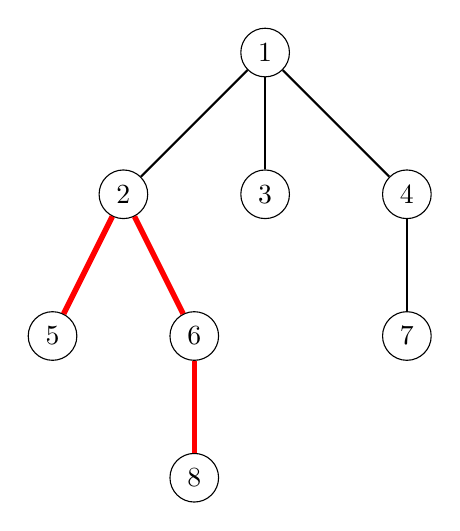
\begin{tikzpicture}[scale=0.9]
        \node[draw, circle] (1) at (0,3) {$1$};
        \node[draw, circle] (2) at (2,1) {$4$};
        \node[draw, circle] (3) at (-2,1) {$2$};
        \node[draw, circle] (4) at (0,1) {$3$};
        \node[draw, circle] (5) at (2,-1) {$7$};
        \node[draw, circle] (6) at (-3,-1) {$5$};
        \node[draw, circle] (7) at (-1,-1) {$6$};
        \node[draw, circle] (8) at (-1,-3) {$8$};
        \path[draw,thick,-] (1) -- (2);
        \path[draw,thick,-] (1) -- (3);
        \path[draw,thick,-] (1) -- (4);
        \path[draw,thick,-] (2) -- (5);
        \path[draw,thick,-] (3) -- (6);
        \path[draw,thick,-] (3) -- (7);
        \path[draw,thick,-] (7) -- (8);

        \path[draw=red,thick,-,line width=2pt] (8) -- node[font=\small] {} (7);
        \path[draw=red,thick,-,line width=2pt] (7) -- node[font=\small] {} (3);
        \path[draw=red,thick,-,line width=2pt] (6) -- node[font=\small] {} (3);
    \end{tikzpicture}
\end{center}

El ancestro común más bajo de los nodos 5 y 8 es el 2. Las profundidades
de los nodos son $\texttt{profundidad}(5)=3$, $\texttt{profundidad}(8)=4$
y $\texttt{profundidad}(2)=2$, por lo que la distancia entre los nodos
5 y 8 es $3+4-2\cdot2=3$.

\section{Algoritmos offline}

Hasta ahora, hemos visto algoritmos \emph{online} para procesar
consultas en árboles. Estos algoritmos son capaces de procesar
consultas una tras otra tal que cada una es realizada antes
de recibir la siguiente consulta.

No obstante, en muchos problemas, la propiedad online no es necesaria.
En esta sección, veremos algoritmos \emph{offline}. Estos algoritmos
reciben un conjunto de consultas que pueden realizarse en cualquier
orden. Usualmente es más fácil diseñar un algoritmo offline que un
algoritmo online.

\subsubsection{Combinar estructuras de datos}

Un método para construir un algoritmo offline es realizar una
búsqueda en profundidad del árbol y mantener estructuras de datos
en los nodos. En cada nodo $s$, creamos una estructura de datos
$\texttt{d}[s]$ que está basada en las estructuras de datos de los
hijos de $s$. Luego, utilizando esta estructura, todas las consultas
relacionadas a $s$ son procesadas.

Por ejemplo, considera el siguiente problema: recibimos un árbol
donde cada nodo posee un valor. Nuestra tarea es procesar consultas
de forma ``calcula el número de nodos con valor $x$ en el subárbol
del nodo $s$''. Por ejemplo, en el siguiente árbol, el subárbol del
nodo $4$ contiene dos nodos cuyos valores son 3.

\begin{center}
    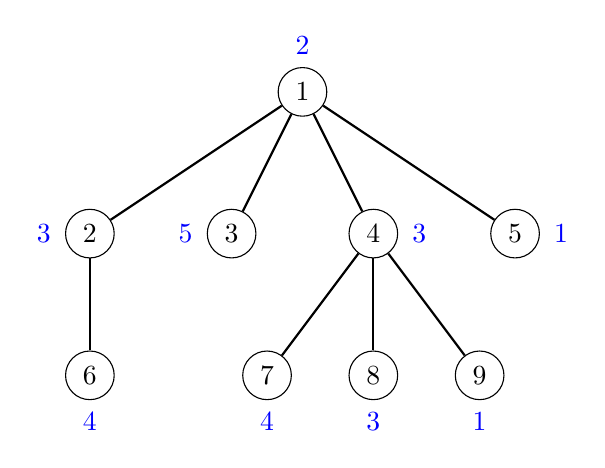
\begin{tikzpicture}[scale=0.9]
        \node[draw, circle] (1) at (0,3) {$1$};
        \node[draw, circle] (2) at (-3,1) {$2$};
        \node[draw, circle] (3) at (-1,1) {$3$};
        \node[draw, circle] (4) at (1,1) {$4$};
        \node[draw, circle] (5) at (3,1) {$5$};
        \node[draw, circle] (6) at (-3,-1) {$6$};
        \node[draw, circle] (7) at (-0.5,-1) {$7$};
        \node[draw, circle] (8) at (1,-1) {$8$};
        \node[draw, circle] (9) at (2.5,-1) {$9$};

        \path[draw,thick,-] (1) -- (2);
        \path[draw,thick,-] (1) -- (3);
        \path[draw,thick,-] (1) -- (4);
        \path[draw,thick,-] (1) -- (5);
        \path[draw,thick,-] (2) -- (6);
        \path[draw,thick,-] (4) -- (7);
        \path[draw,thick,-] (4) -- (8);
        \path[draw,thick,-] (4) -- (9);

        \node[color=blue] at (0,3+0.65) {2};
        \node[color=blue] at (-3-0.65,1) {3};
        \node[color=blue] at (-1-0.65,1) {5};
        \node[color=blue] at (1+0.65,1) {3};
        \node[color=blue] at (3+0.65,1) {1};
        \node[color=blue] at (-3,-1-0.65) {4};
        \node[color=blue] at (-0.5,-1-0.65) {4};
        \node[color=blue] at (1,-1-0.65) {3};
        \node[color=blue] at (2.5,-1-0.65) {1};
    \end{tikzpicture}
\end{center}

En este problema, podemos utilizar estructuras de mapas para resolver
las consultas. Por ejemplo, los mapas para los nodos 4 y sus hijos
son los siguientes:

\begin{center}
    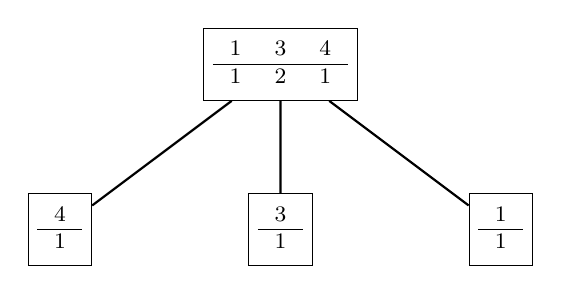
\begin{tikzpicture}[scale=0.7]

        \node[draw, rectangle] (a) at (4,5.5)
        {
            \footnotesize
            \begin{tabular}{rrr}
                4 \\
                \hline
                1 \\
            \end{tabular}};

        \node[draw, rectangle] (b) at (8,5.5)
        {
            \footnotesize
            \begin{tabular}{rrr}
                3 \\
                \hline
                1 \\
            \end{tabular}};

        \node[draw, rectangle] (c) at (12,5.5)
        {
            \footnotesize
            \begin{tabular}{rr}
                1 \\
                \hline
                1 \\
            \end{tabular}};

        \node[draw, rectangle] (d) at (8,8.5)
        {
            \footnotesize
            \begin{tabular}{rrr}
                1 & 3 & 4 \\
                \hline
                1 & 2 & 1 \\
            \end{tabular}};
        \path[draw,thick,-] (a) -- (d);
        \path[draw,thick,-] (b) -- (d);
        \path[draw,thick,-] (c) -- (d);
    \end{tikzpicture}
\end{center}

Si creamos una estructura tal para cada nodo, podemos fácilmente
procesar todas las consultas porque podemos resolver todas las
consultas relacionadas a un nodo inmediatamente después de crear su
estructura de datos. Por ejemplo, el mapa de arriba para el nodo 4
dice que su subárbol contiene dos nodos cuyos valores son 3.

Sin embargo, sería demasiado lento crear todas las estructuras desde cero.
En vez, por cada nodo $s$, creamos una estructura de datos inicial
$\texttt{d}[s]$ que solo contenga el valor de $s$. Luego de esto, podemos
recorrer los hijos de $s$ y \emph{mezclar} $\texttt{d}[s]$ con todas
las estructuras $\texttt{d}[u]$ donde $u$ sea un hijo de $s$.

Por ejemplo, en el árbol de arriba, el mapa para el nodo 4 es creado
mezclando los siguientes mapas:

\begin{center}
    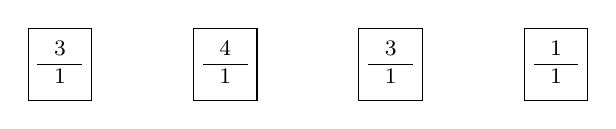
\begin{tikzpicture}[scale=0.7]

        \node[draw, rectangle] (a) at (4,5.5)
        {
            \footnotesize
            \begin{tabular}{rrr}
                4 \\
                \hline
                1 \\
            \end{tabular}};

        \node[draw, rectangle] (b) at (7,5.5)
        {
            \footnotesize
            \begin{tabular}{rrr}
                3 \\
                \hline
                1 \\
            \end{tabular}};

        \node[draw, rectangle] (c) at (10,5.5)
        {
            \footnotesize
            \begin{tabular}{rr}
                1 \\
                \hline
                1 \\
            \end{tabular}};

        \node[draw, rectangle] (d) at (1,5.5)
        {
            \footnotesize
            \begin{tabular}{rr}
                3 \\
                \hline
                1 \\
            \end{tabular}};

    \end{tikzpicture}
\end{center}

Aquí el primer mapa es la estructura de datos inicial para el nodo 4,
y los otros tres mapas corresponden a los nodos 7, 8, y 9.

La mezcla en el nodo $s$ puede hacerse de la siguiente manera:
Visitamos todos los hijos de $s$ y por cada hijo $u$ mezclamos
$\texttt{d}[s]$ con $\texttt{d}[u]$. Siempre copiamos los contenidos
de $\texttt{d}[u]$ a $\texttt{d}[s]$. Antes de esto, \emph{intercambiamos}
los contenidos de $\texttt{d}[s]$ y $\texttt{d}[u]$ si $\texttt{d}[s]$
es más pequeño que $\texttt{d}[u]$. Al hacer esto, cada valor es copiado
solamente $O(\log n)$ veces durante el recorrido del árbol, lo que
asegura que el algoritmo es eficiente.

Para intercambiar los contenidos de dos estructuras de datos $a$ y $b$
eficientemente, podemos simplemente usar el siguiente código:

\begin{lstlisting}
swap(a, b);
\end{lstlisting}

Está garantizado que el código de arriba funciona en tiempo constante
donde $a$ y $b$ son estructuras de datos de la librería estándar de C++.

\subsubsection{Ancestro común más bajo}

También existe un algoritmo offline para procesar un conjunto de
consultas del ancestro común más bajo.\footnote{Este algoritmo
    fue publicado por R. E. Tarjan en 1979 \cite{tar79}.} El algoritmo
está basado en la estructura de unión--búsqueda (ver Capítulo 15.2),
y el beneficio del algoritmo es su facilidad de implementación sobre
los otros algoritmos que vimos hasta ahora.

El algoritmo recibe un conjunto de pares de nodos y determina,
por cada tal par, su ancestro común más bajo. El algoritmo realiza una
búsqueda en profundidad y mantiene conjuntos disjuntos de nodos.
Inicialmente, cada nodo pertenece a un conjunto diferente. Por cada
conjunto, también almacenamos el nodo más alto en el árbol que
pertenezca al conjunto.

Cuando el algoritmo visita un nodo $x$, recorre todos los nodos $y$
tal que el ancestro común más bajo de $x$ e $y$ deba ser encontrado.
Si $y$ ya se ha visitado, el algoritmo reporta que el ancestro común
más bajo de $x$ e $y$ es el nodo más alto en el conjunto de $y$.
Tras procesar el nodo $x$, se unen los conjuntos de $x$ y su padre.

Por ejemplo, supongamos que queremos encontrar el ancestro común
más bajo de los pares de nodos $(5,8)$ y $(2,7)$ en el siguiente árbol:
\begin{center}
    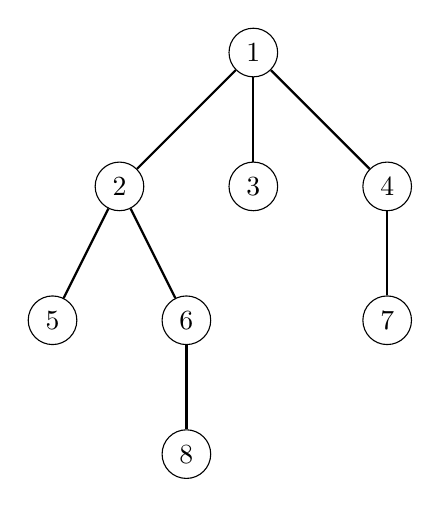
\begin{tikzpicture}[scale=0.85]
        \node[draw, circle] (1) at (0,3) {$1$};
        \node[draw, circle] (2) at (2,1) {$4$};
        \node[draw, circle] (3) at (-2,1) {$2$};
        \node[draw, circle] (4) at (0,1) {$3$};
        \node[draw, circle] (5) at (2,-1) {$7$};
        \node[draw, circle] (6) at (-3,-1) {$5$};
        \node[draw, circle] (7) at (-1,-1) {$6$};
        \node[draw, circle] (8) at (-1,-3) {$8$};
        \path[draw,thick,-] (1) -- (2);
        \path[draw,thick,-] (1) -- (3);
        \path[draw,thick,-] (1) -- (4);
        \path[draw,thick,-] (2) -- (5);
        \path[draw,thick,-] (3) -- (6);
        \path[draw,thick,-] (3) -- (7);
        \path[draw,thick,-] (7) -- (8);
    \end{tikzpicture}
\end{center}

En los siguientes árboles, los nodos grises denotan nodos visitados
y los grupos punteados de nodos pertenecen al mismo conjunto.
Cuando el algoritmo visita el nodo 8, se da cuenta de que el nodo 5
se ha visitado y el nodo más alto en su conjunto es 2. Por ende, el
ancestro común más bajo de los nodos 5 y 8 es 2:
\begin{center}
    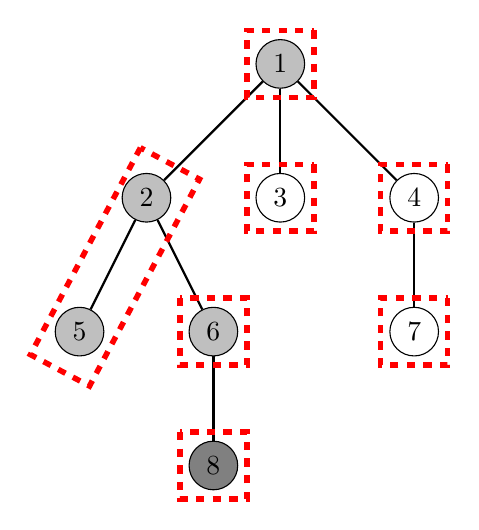
\begin{tikzpicture}[scale=0.85]
        \node[draw, circle, fill=lightgray] (1) at (0,3) {$1$};
        \node[draw, circle] (2) at (2,1) {$4$};
        \node[draw, circle, fill=lightgray] (3) at (-2,1) {$2$};
        \node[draw, circle] (4) at (0,1) {$3$};
        \node[draw, circle] (5) at (2,-1) {$7$};
        \node[draw, circle, fill=lightgray] (6) at (-3,-1) {$5$};
        \node[draw, circle, fill=lightgray] (7) at (-1,-1) {$6$};
        \node[draw, circle, fill=gray] (8) at (-1,-3) {$8$};
        \path[draw,thick,-] (1) -- (2);
        \path[draw,thick,-] (1) -- (3);
        \path[draw,thick,-] (1) -- (4);
        \path[draw,thick,-] (2) -- (5);
        \path[draw,thick,-] (3) -- (6);
        \path[draw,thick,-] (3) -- (7);
        \path[draw,thick,-] (7) -- (8);

        \draw [red,thick,dashed,line width=2pt,rotate around={-28:(-2,0)}] (-2.9,1.5) rectangle (-1.9,-2);


        \draw [red,thick,dashed,line width=2pt] (-1.5,-0.5) rectangle (-0.5,-1.5);
        \draw [red,thick,dashed,line width=2pt] (-1.5,-2.5) rectangle (-0.5,-3.5);

        \draw [red,thick,dashed,line width=2pt] (0.5,3.5) rectangle (-0.5,2.5);
        \draw [red,thick,dashed,line width=2pt] (0.5,1.5) rectangle (-0.5,0.5);
        \draw [red,thick,dashed,line width=2pt] (2.5,1.5) rectangle (1.5,0.5);
        \draw [red,thick,dashed,line width=2pt] (2.5,-0.5) rectangle (1.5,-1.5);
    \end{tikzpicture}
\end{center}

Más tarde, al visitar el nodo 7, el algoritmo determina que el ancestro
común más bajo de los nodos 2 y 7 es 1:
\begin{center}
    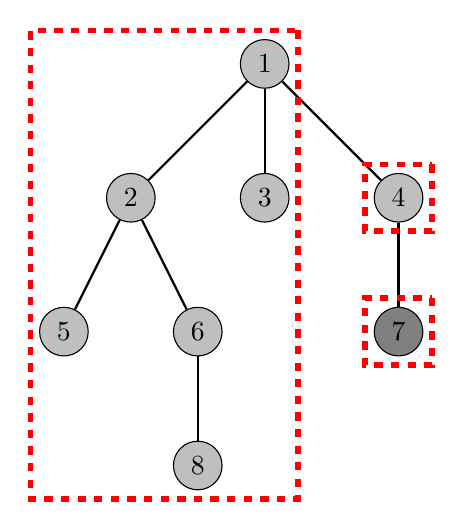
\begin{tikzpicture}[scale=0.85]
        \node[draw, circle, fill=lightgray] (1) at (0,3) {$1$};
        \node[draw, circle, fill=lightgray] (2) at (2,1) {$4$};
        \node[draw, circle, fill=lightgray] (3) at (-2,1) {$2$};
        \node[draw, circle, fill=lightgray] (4) at (0,1) {$3$};
        \node[draw, circle, fill=gray] (5) at (2,-1) {$7$};
        \node[draw, circle, fill=lightgray] (6) at (-3,-1) {$5$};
        \node[draw, circle, fill=lightgray] (7) at (-1,-1) {$6$};
        \node[draw, circle, fill=lightgray] (8) at (-1,-3) {$8$};
        \path[draw,thick,-] (1) -- (2);
        \path[draw,thick,-] (1) -- (3);
        \path[draw,thick,-] (1) -- (4);
        \path[draw,thick,-] (2) -- (5);
        \path[draw,thick,-] (3) -- (6);
        \path[draw,thick,-] (3) -- (7);
        \path[draw,thick,-] (7) -- (8);

        \draw [red,thick,dashed,line width=2pt] (0.5,3.5) rectangle (-3.5,-3.5);
        \draw [red,thick,dashed,line width=2pt] (2.5,1.5) rectangle (1.5,0.5);
        \draw [red,thick,dashed,line width=2pt] (2.5,-0.5) rectangle (1.5,-1.5);

    \end{tikzpicture}
\end{center}
